\chapter{Diseño e implementación}
La aplicación recopila información del usuario en distintas etapas. Se trata de una aplicación web que ejecuta código tanto en cliente como en servidor para obtener dicha información.
\begin{itemize}
    \item \textbf{Cliente}: Es la parte de la aplicación ejecutada en el navegador del usuario. Obtiene información del navegador mediante código JavaScript y lo envía al servidor de forma asíncrona.
    \item \textbf{Servidor}: Aloja la base de datos y el código que obtiene la información de las cabeceras HTTP.
     \begin{itemize}
         \item \textbf{Base de datos}: Una base de datos relacional MariaDB/MySQL en la que se almacenarán los datos obtenidos de cada una de las conexiones de los usuarios.
     \end{itemize}
\end{itemize}
\section{Funcionamiento}
\begin{figure}[tbp]
    \centering
    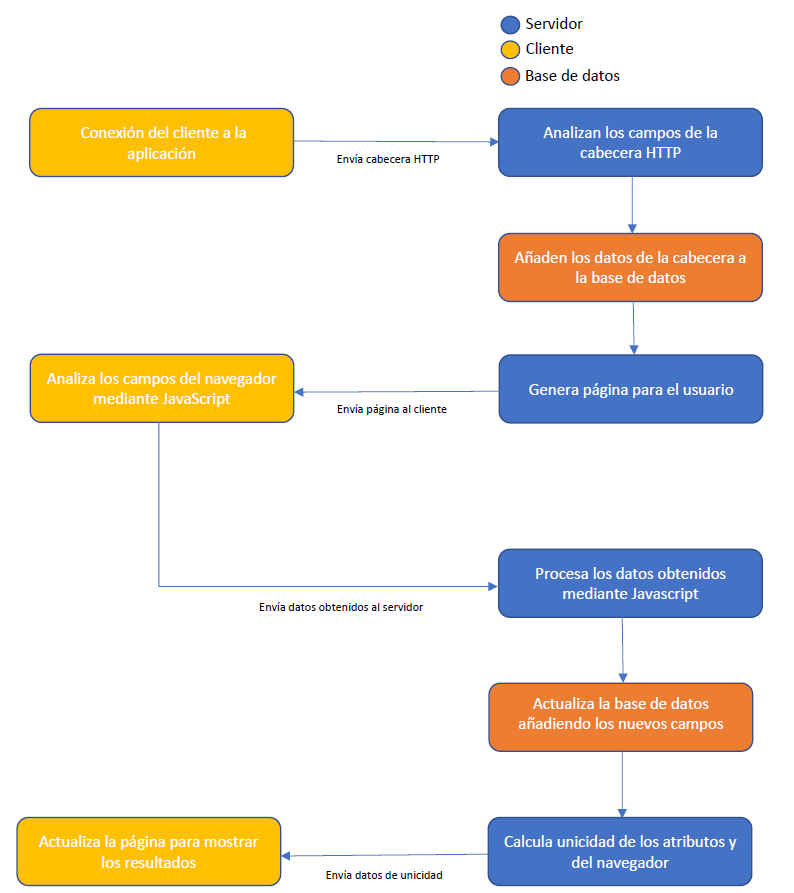
\includegraphics[width=1\textwidth]{Images/diagrama flujo.png}
    \caption{Diagrama de flujo de la aplicación}
    \label{fig:diagramaFlujo}
\end{figure}
Nuestra aplicación se ejecuta tanto en cliente como en servidor, en distintas etapas y comunicándose de manera asíncrona en algunas de ellas. \par
El cliente hace una petición HTTP al servidor. El servidor analiza las cabeceras de la petición y las inserta en la base de datos con un identificador asociado al usuario para definir su huella. Devuelve al usuario una página estática en HTML con JavaScript embebido en la que el usuario verá los datos de su cabecera HTTP y el código JavaScript se ejecutará automáticamente para obtener el resto de datos del navegador. \\
Una vez terminada la ejecución de todo el código JavaScript, este actualizará la apariencia de la página para que el usuario pueda ver las características obtenidas mediante JavaScript y enviará de forma asíncrona, sin recargar la página del usuario, toda la información obtenida al servidor. \\
El servidor recibe la información obtenida en JavaScript y actualiza todas las filas de las tablas de la base de datos para el id del usuario. \\
Por último, el servidor ejecuta el código encargado de calcular la unicidad de cada uno de los atributos del usuario por separado y la unicidad total del conjunto de atributos. Tras calcularlo devolverá como respuesta de la petición asíncrona del código JavaScript todos los valores de la unicidad, que volverán a actualizar la página para mostrarle al usuario cuánto de único es en cada uno de los campos de su navegador y cuánto de único es su navegador en conjunto.
\section{Componentes del sistema}
El proyecto cuenta con distintos componentes. Principalmente se dividen en cliente y servidor.
\subsection{Servidor}
El servidor se encarga de gestionar las peticiones HTTP enviadas por el usuario al utilizar nuestra aplicación web.\par
La página consta de dos rutas, que serán generadas por el servidor mediante PHP:
\begin{itemize}
    \item \textbf{/}: Es la base de la aplicación. En ella se analizan y muestran todos los elementos del navegador del usuario, así como su unicidad general e individual de cada uno de los atributos del navegador.
    \item \textbf{/graficas}: En esta página se muestra al usuario gráficas con los datos globales de los atributos obtenidos por la aplicación.
\end{itemize}
Para la funcionalidad principal de la aplicación el servidor actúa en dos ocasiones. \par
La primera se encarga de recopilar la información de la cabecera HTTP, generar la página que verá el usuario e insertar en la base de datos esta información. Esta parte corresponde a la ruta principal. \par 
La segunda ocasión recibe una petición asíncrona con los datos obtenidos en la ejecución de código en cliente. El servidor se encarga de actualizar la base de datos añadiendo esos datos a las tablas para el id del usuario. Una vez añadida esta información, genera un objeto JSON que devolverá como respuesta de la petición. En este objeto se encuentra la unicidad de cada uno de los elementos analizados y la unicidad general del navegador del usuario. Esta acción se lleva a cabo haciendo una llamada a la ruta /cargaJS.
\subsubsection{Lenguaje de programación}
Para el código del servidor hemos utilizado el lenguaje PHP. Con él se gestiona todo el funcionamiento de la aplicación en el servidor.\par
En el servidor se generan las páginas HTML que se envían al cliente. Al ser necesario que cada cliente reciba una página única y personalizada éstas se generan de manera dinámica en el servidor con este lenguaje. Por otra parte, PHP nos permite obtener la información de la cabecera HTTP que recibe el servidor y tratarla para añadir esta información en la página que verá el cliente y a su vez insertarla en nuestra base de datos.\par
\newpage
\subsubsection{Base de datos}
La base de datos de nuestra aplicación es de tipo relacional. Consta de 5 tablas, en la que la tabla principal es la tabla \textit{Conexiones}. En la figura \ref{fig:diagramaEntidadRelacion} se puede observar el diagrama entidad-relación de nuestra base de datos, en el que omitimos muchos los atributos de las tablas al ser su número tan elevado que dificultaría la legibilidad del diagrama.
\begin{figure}[tbp]
    \centering
    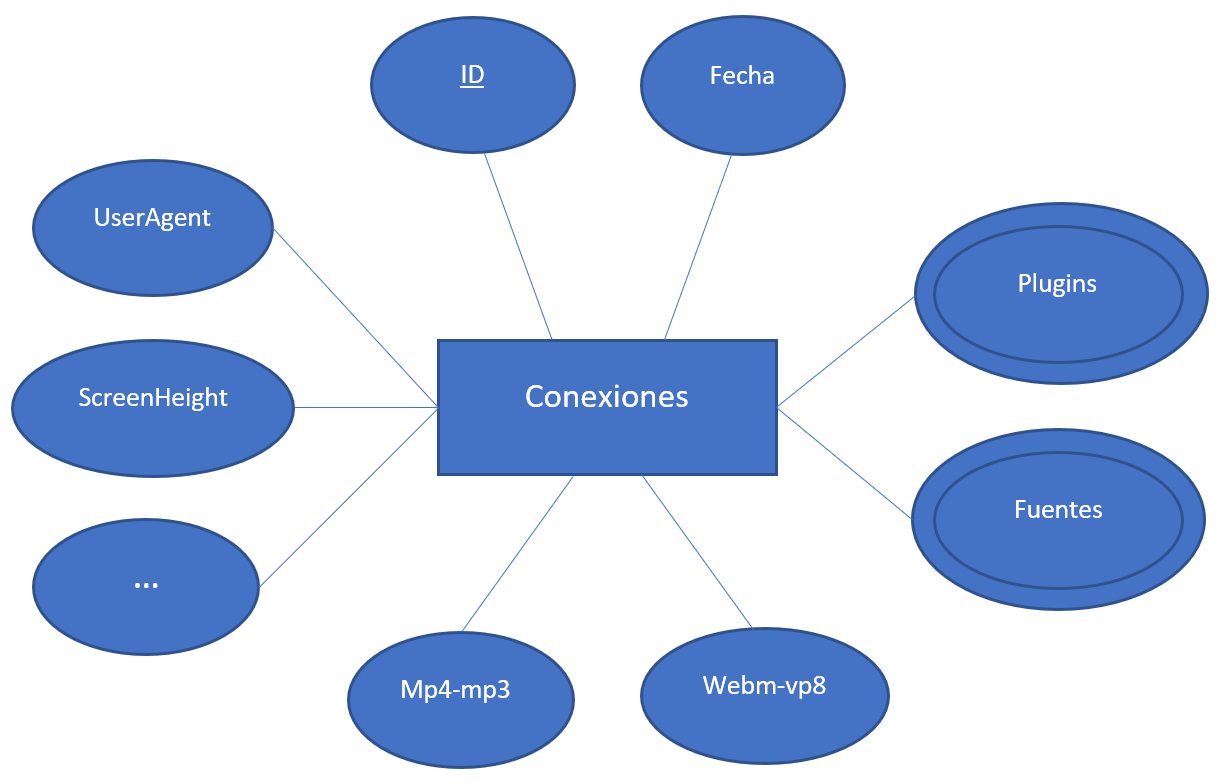
\includegraphics[width=1\textwidth]{Images/entidad relacion.png}
    \caption{Diagrama entidad-relación de la base de datos}
    \label{fig:diagramaEntidadRelacion}
\end{figure}
A continuación detallaremos las tablas de nuestra base de datos.
\begin{itemize}
    \item \textbf{Conexiones}: La tabla principal de la base de datos. En ella se almacenan el ID del usuario, la fecha de la inserción, los datos obtenidos de la cabecera HTTP (detallados en la tabla \ref{tab:resultadosHTTP}) y la mayoría de atributos obtenidos mediante JavaScript (tabla \ref{tab:resultadosJavascript}).
    El ID es la clave primaria de la tabla e identifica al usuario y a todos sus atributos.\par
    Los atributos de la cabecera HTTP varían en los distintos navegadores o incluso en un mismo navegador. Por esa razón examinamos los atributos de las cabeceras HTTP de distintos navegadores y en distintos dispositivos, y seleccionamos los mas comunes para insertarlos en la base de datos. Estos elementos se detallan en la tabla \ref{tab:resultadosHTTP}. El resto de elementos se pueden observar en la aplicación, pero no los almacenamos.\par
    La fecha se almacena por seguridad y estaba pensado utilizarla en una opción para comprobar las huellas almacenadas en distintos intervalos de tiempo, funcionalidad que ha quedado como trabajo futuro. \par
    \begin{table}[tbp]
        \centering
        \begin{tabular}{c|c}
            \textbf{Atributo} & \textbf{Tipo} \\ \hline
            \underline{ID} & Int \\
            Fecha & Timestamp \\
            Accept & Varchar\\
            AcceptLanguage & Varchar\\
            UpgradeInsecureRequest & Varchar\\
            UserAgent & Varchar\\
            AcceptEncoding & Varchar\\
            Connection & Varchar\\
            SecFetchMode & Varchar\\
            SecFetchUser & Varchar\\
            SecFetchSite & Varchar\\
            DNT & TinyInt\\
        \end{tabular}
        \caption{Atributos de la cabecera HTTP en la tabla \textit{Conexiones}}
        \label{tab:resultadosHTTP}
    \end{table}
    El resto de atributos de la tabla \textit{Conexiones} son los obtenidos mediante JavaScript. Estos elementos están detallados en la tabla \ref{tab:resultadosJavascript}.\newpage
    \begin{table}[tbp]
        \begin{minipage}[c]{85mm}
        \centering
            \begin{tabular}{c|c}
                \textbf{Atributo} & \textbf{Tipo} \\ \hline
                Plataforma & Varchar\\
                UserAgentJS & Varchar\\
                Navegador & Varchar\\
                Version & Int\\
                CookieEnabled & TinyInt\\
                Language & Varchar\\
                Lenguajes & Varchar\\
                OnLine & TinyInt\\
                AppName & Varchar\\
                Bateria & TinyInt\\
                DNTJS & TinyInt\\
                TouchPoints & Int\\
                Product & Varchar\\
                ProductSub & Varchar\\
                OS & Varchar\\
                Vendor & Varchar\\
                HardwareConcurrency & Int\\
                BuildID & Varchar\\
                DevMemory & Float\\
                ResumenPlugins & Varchar\\
            \end{tabular}
        \end{minipage}
        \begin{minipage}[c]{45mm}
        \centering
            \begin{tabular}{c|c}
                \textbf{Atributo} & \textbf{Tipo} \\ \hline
                ZonaHoraria & Int\\
                ScreenWidth & Int\\
                ScreenHeight & Int\\
                ScreenAvailWidth & Int\\
                ScreenAvailHeigth & Int\\
                ScreenColorDepth & Int\\
                ScreenPixelDepth & Int\\
                LocationBar & TinyInt\\
                PixelRatio & Double\\
                MenuBar & TinyInt\\
                PersonalBar & TinyInt\\
                StatusBar & TinyInt\\
                ToolBar & TinyInt\\
                LocalStorage & TinyInt\\
                SessionStorage & TinyInt\\
                IndexDB & TinyInt\\
                WindowResults & TinyInt\\
                Canvas & Varchar\\
                ResumenFuentes & Varchar\\
            \end{tabular}
        \end{minipage}
        \caption{Atributos obtenidos mediante JavaScript en la tabla \textit{Conexiones}}
        \label{tab:resultadosJavascript}
    \end{table}
    Entre los atributos de JavaScript destacan tres en concreto:
    \begin{itemize}
        \item \textbf{Canvas}: Es el resumen del resultado del elemento \textit{canvas} dibujado en el navegador. Este elemento se puede leer como una cadena de caracteres de una longitud considerable. Por ello decidimos resumirla utilizando el algoritmo <<MD5>> para almacenarla en la base de datos sin ocupar tanto espacio.
        \item \textbf{ResumenFuentes}: Se trata de un resumen utilizando el algoritmo <<MD5>> de todas las fuentes detectadas en el navegador. Para ello, a la hora de almacenar las fuentes, también las ordenamos y concatenamos, para después resumirlas e insertarlas en esta tabla. Esto se hace para ahorrar tiempo a la hora de calcular la unicidad de la huella del usuario.
        \item \textbf{ResumenPlugins}: Hacemos un resumen de todos los plugins encontrados en el navegador de la misma forma que hacemos con las fuentes y por la misma razón. Para el resumen de este elemento también utilizamos el algoritmo <<MD5>>.
    \end{itemize}
    \item \textbf{FormatosAudio}: En esta tabla se almacenan los resultados de la comprobación de los distintos formatos de audio soportados por el navegador. Para hacer esta comprobación analizamos los formatos mas comunes en la actualidad en navegadores \cite{Formatos}. Estos elementos forman parte de la tabla \textit{Conexiones}, pero decidimos almacenarlos en una tabla alternativa para trabajar con conjuntos de elementos mas reducidos. En la tabla \ref{tab:formatosAudio} se detallan los atributos de esta.\par
    \item \textbf{FormatosVideo}: En esta tabla se almacenan los resultados de la comprobación de los distintos formatos de vídeo soportados por el navegador. De la misma forma que con los formatos de audio, analizamos los formatos de vídeo mas comunes en navegadores \cite{Formatos}. Por el mismo motivo que en la tabla \textit{FormatosAudio}, decidimos almacenar los resultados de los formatos de vídeo en una tabla aparte.Se pueden ver en detalle sus atributos en la tabla \ref{tab:formatosVideo}\par
    \begin{table}[tbp]
    \centering
        \begin{minipage}[c]{70mm}
        \centering
            \begin{tabular}{c|c}
                \textbf{Columna} & \textbf{Tipo} \\ \hline
                ogg-vorbis & Varchar\\
                3gpp & Varchar\\
                mp4-mp4a & Varchar\\
                mp4-mp3 & Varchar\\
                mp4-ac3 & Varchar\\
                mp4-ec3 & Varchar\\
                acc & Varchar\\
                pcm & Varchar\\
                mpeg & Varchar\\
                flac & Varchar\\
                wave & Varchar\\
                webm-vorbis & Varchar\\
                mp3-mp3 & Varchar\\
            \end{tabular}
            \caption{Tabla \textit{FormatosAudio}}
            \label{tab:formatosAudio}
        \end{minipage}
        \begin{minipage}[c]{70mm}
        \centering
            \begin{tabular}{c|c}
                \textbf{Columna} & \textbf{Tipo} \\ \hline
                ogg-theora & Varchar\\
                ogg-vorbis & Varchar\\
                ogg-opus & Varchar\\
                mp4-avc1 & Varchar\\
                mp4-mp4a & Varchar\\
                mp4-flac & Varchar\\
                webm-vp8 & Varchar\\
                webm-vp9 & Varchar\\
                webm-vorbis & Varchar\\
            \end{tabular}
            \caption{Tabla \textit{FormatosVideo}}
            \label{tab:formatosVideo}
        \end{minipage}
    \end{table}
    \item \textbf{Plugins}: En esta tabla se almacenan los nombres de los plugins encontrados en un navegador. Se trata de un atributo multivaluado de la tabla \textit{Conexiones}. Los atributos de esta tabla están detallados en la tabla \ref{tab:plugins}.
    \newpage
    \item \textbf{Fuentes}: Tabla en la que se almacenan todos los nombres de las fuentes encontradas en el navegador del usuario.En ella se guardan todas las fuentes encontradas en cada análisis del navegador. Es un atributo multivaluado de la tabla \textit{Conexiones}. Sus atributos se detallan en la tabla \ref{tab:fuentes}.
    \begin{table}[h]
    \centering
        \begin{minipage}[c]{70mm}
        \centering
            \begin{tabular}{c|c}
                \textbf{Columna} & \textbf{Nombre} \\ \hline
                \underline{ID} & Int \\
                \underline{NombrePlugin} & Varchar\\
            \end{tabular}
            \caption{Columnas de la tabla \textit{Plugins}}
            \label{tab:plugins}
        \end{minipage}
        \begin{minipage}[c]{70mm}
        \centering
            \begin{tabular}{c|c}
                \textbf{Columna} & \textbf{Nombre} \\ \hline
                \underline{ID} & Int \\
                \underline{NombreFuente} & Varchar\\
            \end{tabular}
            \caption{Columnas de la tabla \textit{Fuentes}}
            \label{tab:fuentes}
        \end{minipage}
    \end{table}
\end{itemize}
\subsection{Cliente}
En cliente se carga la página del usuario, en la que se muestran los datos del navegador en el que se está ejecutando la aplicación.\par
La página que recibe el usuario es dinámica. Al principio en ella se muestra la información obtenida de la cabecera HTTP mientras se ejecuta código JavaScript encargado de obtener el resto de datos del navegador. Cuando se termina de ejecutar esta parte, se realiza una llamada asíncrona al servidor, en la que se envían todos los datos obtenidos y la página queda a la espera de la respuesta de este. Al recibir la respuesta en la que se encuentran todos los valores de la unicidad del navegador, se actualiza la apariencia de la página para que el usuario pueda terminar de ver toda la información relacionada a su navegador y cuánto de única es su huella. 
\subsubsection{Lenguajes de programación}
El lenguaje utilizado en cliente para generar la página es HTML, con JavaScript para toda la parte dinámica.\par
El código JavaScript se encarga de obtener datos del navegador mediante clases y funciones predefinidas en el JavaScript y otros métodos desarrollados por nosotros. Además JavaScript nos permite realizar las peticiones asíncronas al servidor de forma que se puede actualizar la página sin necesidad de recargarla una vez recibe la respuesta del servidor.\par 
Para la generación de los gráficos de las estadísticas de la aplicación utilizamos la herramienta <<Google Charts>> \cite{GoogleCharts}, la cual importamos mediante JavaScript y que permite crear distintos tipos de gráficas.
\newpage
\section{Problemas}
Durante el desarrollo de la aplicación nos hemos encontrado con distintos problemas, los cuales detallaremos a continuación junto con las soluciones que hemos encontrado para estos.
\subsubsection{Asincronía}
Este problema surgió durante la implementación de la parte asíncrona de nuestra aplicación. Para la realización de esta utilizamos el objeto  <<XMLHTTPRequest>> de JavaScript. Este permite realizar peticiones al servidor mientras se sigue ejecutando código en cliente y, una vez recibe la respuesta del servidor, puede ejecutar funciones que estaban a la espera de la respuesta. El código JavaScript que utilizamos está dividido en distintas secciones, dependiendo de los objetos que se utilizan o el tipo de información que se obtiene. Una vez se termina de obtener todos los datos de cada sección se realiza el envío de información al servidor de esa parte. Solo en el último envío, cuando ya están todos los datos alojados en el servidor se espera la información devuelta por este para actualizar la página.\par 
Al ejecutarse el código de manera asíncrona en el servidor, en algunas ocasiones se ejecutaba la última petición antes que el resto, por lo que se retornaba una unicidad errónea del navegador, ya que se recibía la respuesta antes de que el resto de datos hubiesen sido añadidos en el servidor.\par 
Para solucionarlo hicimos que una vez lanzada una petición asíncrona no lanzase la siguiente hasta haber recibido la respuesta del servidor, de forma que se lanzasen síncronamente.
\subsubsection{Campos de cabeceras HTTP}
Los elementos de la cabecera HTTP pueden variar de un navegador a otro, e incluso dentro de un mismo navegador. Nuestra aplicación analiza todos los campos de la cabecera HTTP de manera automática, por lo que en ocasiones pueden aparecer elementos con los que no contamos.\par 
La solución fue analizar los elementos mas comunes a todos los navegadores y controlar que solo fuesen esos los que tratamos dentro de la aplicación. Esta comprobación la hacemos mediante PHP en el servidor. El resto de datos solo se muestran en la página al usuario para comprobar los elementos que conforman la cabecera HTTP de su navegador.
\subsubsection{Campos multivaluados}
En nuestra base de datos existen dos tablas que corresponden a atributos multivaluados de la tabla \textit{Conexiones}. Estas tablas son \textit{fuentes} y \textit{plugins}. En estas tablas se almacenan en cada fila un nombre de fuente o plugin y el ID del resultado al que pertenecen. El problema surgió a la hora de comprobar la unicidad de la huella del usuario, ya que se complicaba la consulta a realizar por la cantidad de filas de la tabla.\par
La solución que encontramos fue añadir un resumen de estos elementos en la tabla \textit{Conexiones}. Para ello, además de insertar todos los elementos de fuentes y plugins en sus respectivas tablas, concatenamos estos elementos ordenados y los resumimos. De esta forma se simplificaba mucho el cálculo de la unicidad de la huella del usuario.